%!TEX root = report.tex
\chapter{WebApp for Active Delay Warning}
\label{ch:mobile_app}

\par We designed a web application to demonstrate the potential use of our API data service. It allows users to search for nearby bus stops, view the available routes and live bus arrival times. For each route, the user can view the historical, current and reference bus travel time to reach each downstream bus stop.

\section{Implementation}
\subsection{AugularJS Framework}
\par We chose to use the AngularJS Framework \cite{angularjs} with UI Bootstrap \cite{bootstrap} to build the front-end of the application. This was because AngularJS employs a clear Model-View-Controller structure, and has a wide range of packages to build extensions with. We used \texttt{Google Maps API} \cite{angular_google_maps} and \texttt{ui-router} \cite{ui_router} extensively.

\subsection{Development \& Deployment Pipeline}
\par We used Yeoman \cite{yeoman}, a web application scaffolding tool, to organise and manage scripts and files. We also used Grunt \cite{grunt}, a Javascript task runner to manage the build and deployment process.

\par For deployment, we created a Grunt task to run tests, minify the javascript files, and copy the minified version to the production server.

\section{Front-end User Guide}
\par The web application has a simple user interface. It divides the screen space into 2 parts, the top half consists of a map area, and the bottom half an information panel. We deployed the front-end web to \url{http://delay.doc.ic.ac.uk/}.

\subsection{Landing Page}

\begin{figure}
\centering
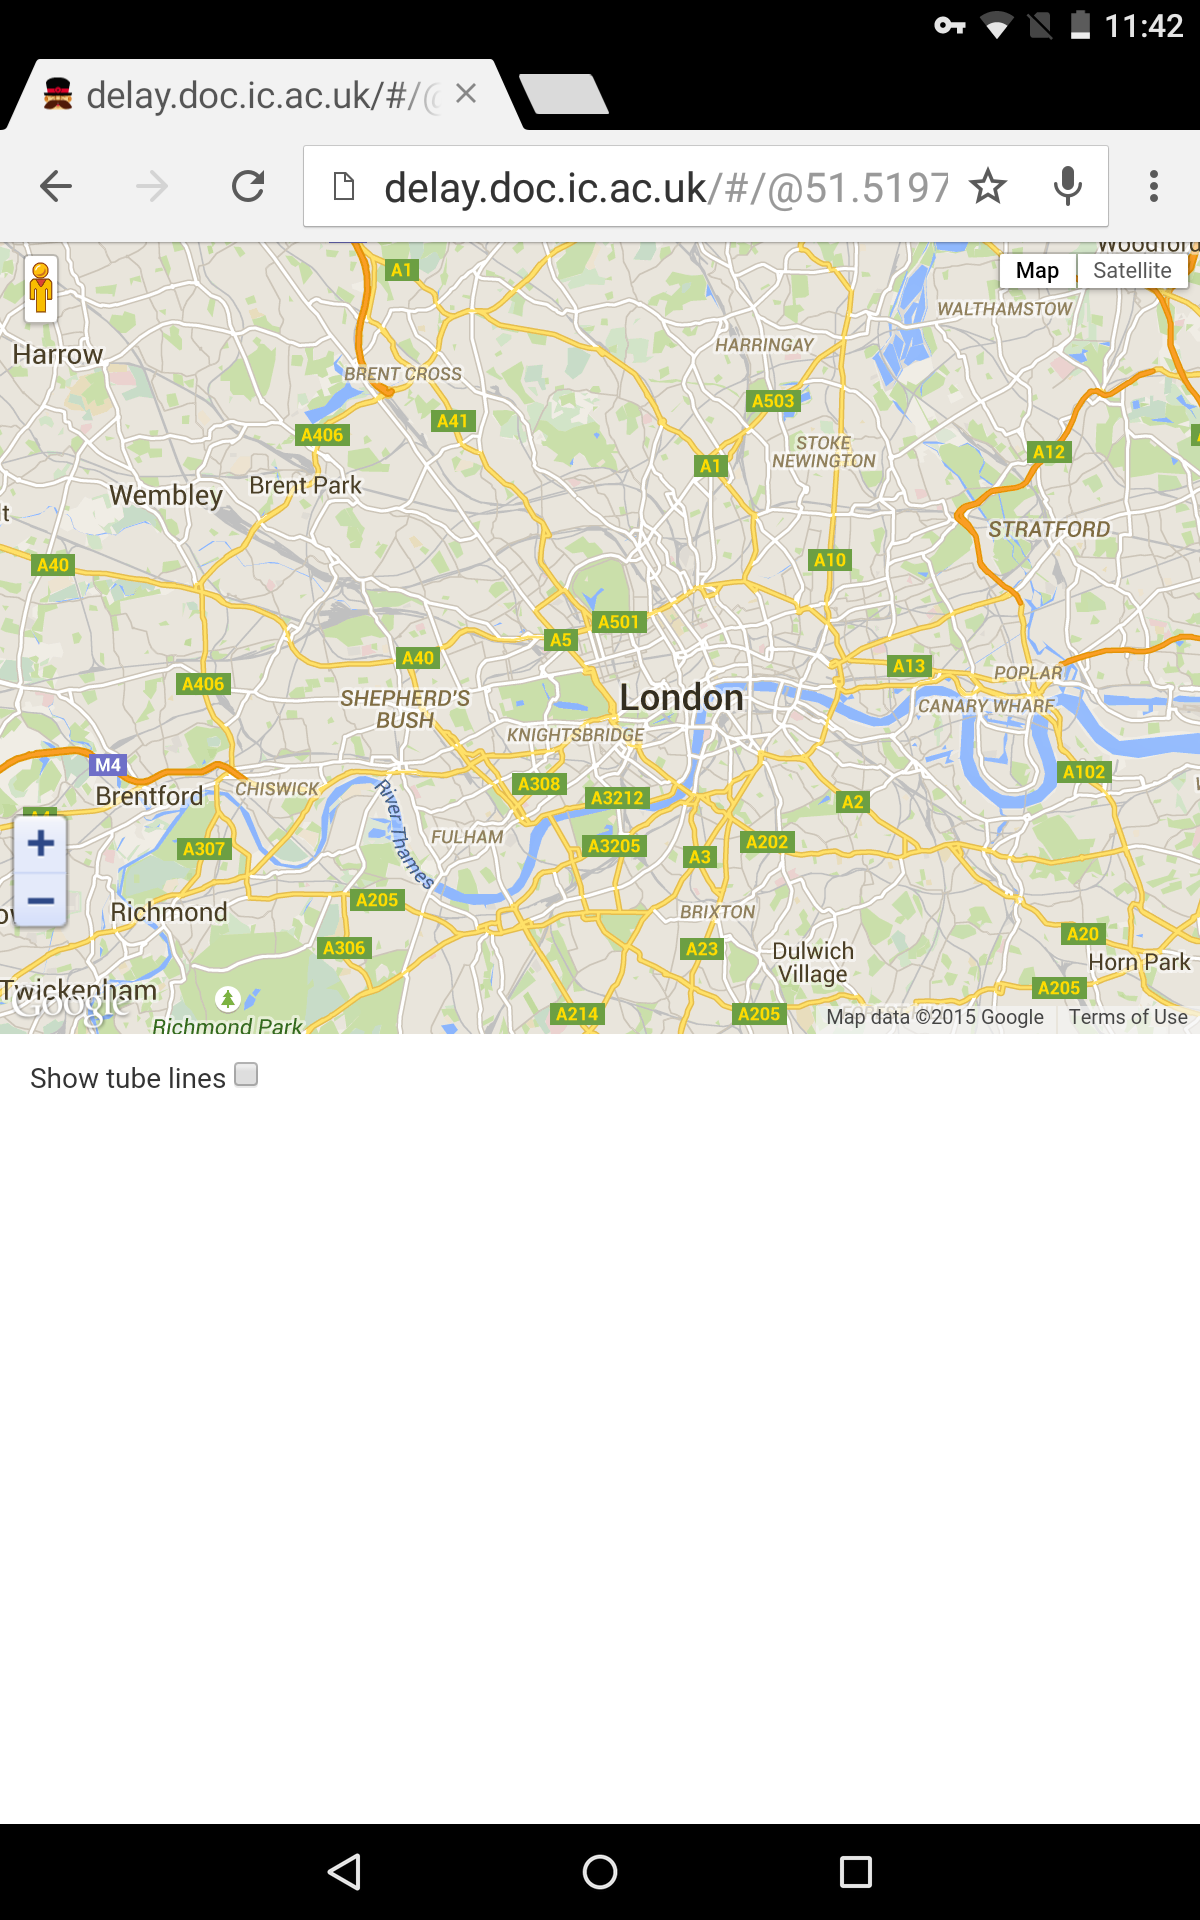
\includegraphics[width=0.8\textwidth]{figures/landing_page.png}
\caption{\label{fig:landing_page} Web Application Langding Page}
\end{figure}

\par On load, the app will attempt to obtain the current location of the device, and centre the map on it. If the current location is not available, then the default map centred on London will be loaded (Figure \ref{fig:landing_page}).


\subsection{Nearby Bus Stops Arrival}

\begin{figure}
\centering
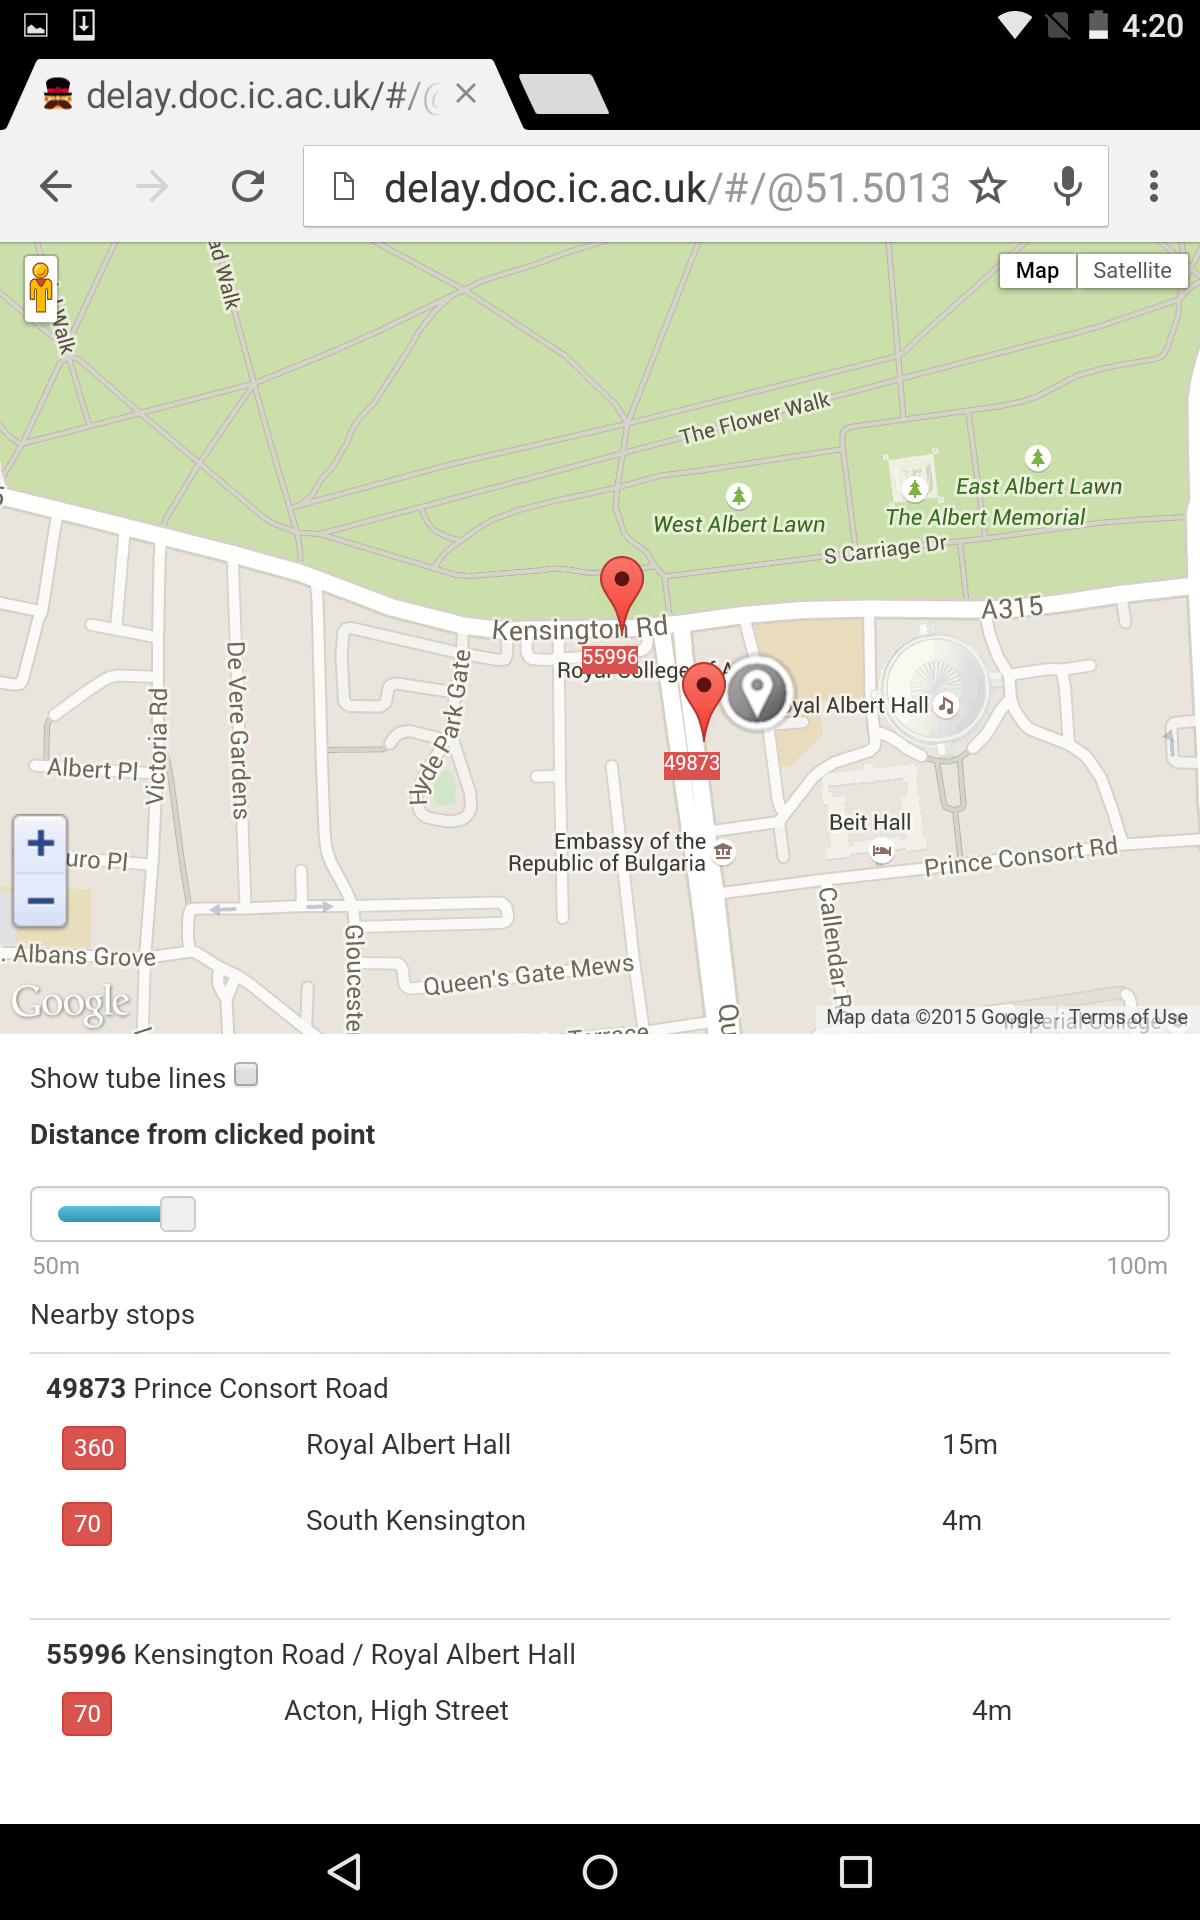
\includegraphics[width=0.8\textwidth]{figures/clicked_view.png}
\caption{\label{fig:clicked_view} Web Application Nearby Bus Stops}
\end{figure}

\par A click on the map will place a grey location marker and make a request to the \texttt{arrivals} endpoint to search for the nearby bus stops within a given radius. The default radius is 100 meters. Users can use the slider to change the radius of the search area, ranging from 50 to 500 meters.

\par A list of the nearby bus stops and the routes available at each stop will be shown in the information panel, with the \acrshort{tfl} bus arrivals displayed at the side showing the arrival times for the incoming buses(Figure \ref{fig:clicked_view}). For each bus stop, a red marker will be placed in the map at the stop location with the stop code displayed under the marker.

\subsection{Bus Delay Predictions}
\begin{figure}
\centering
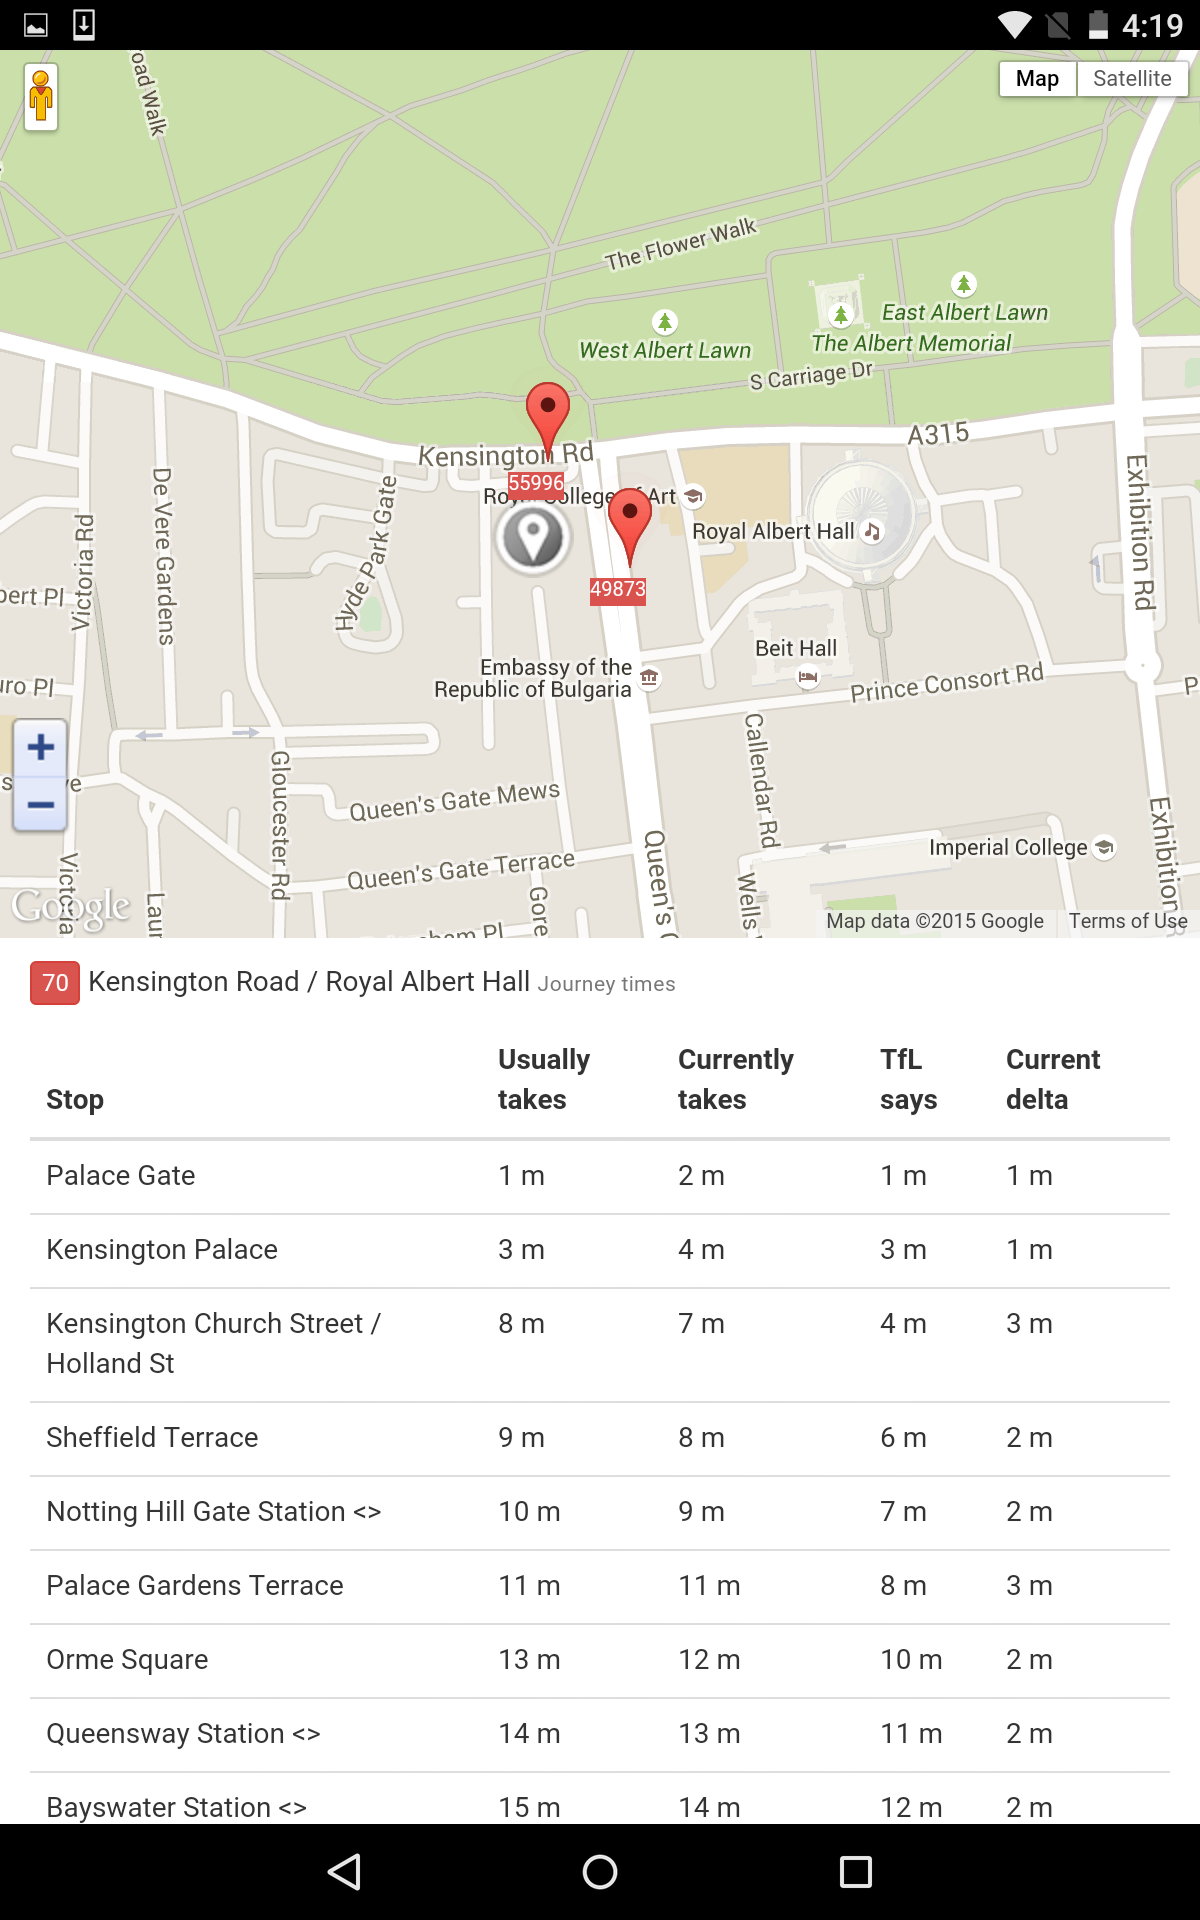
\includegraphics[width=0.8\textwidth]{figures/timetables.png}
\caption{\label{fig:timetable_view} Web Application Timetables for a Route}
\end{figure}

\par For each available route at a nearby bus stop, users could check the historical, current, and reference travel time to each downstream stops by clicking the red button to select a specific route for details. The app will make requests to the \texttt{Historical \& Current} and \texttt{Reference} endpoints with the current day of the week, hour of the day, stop code, and direction of the bus route as parameters.

\par After the endpoints return results, a list of the downstream stops with the corresponding historical, current, and reference travel time from the current stop will be displayed in the information panel. The \texttt{current - ref} column indicates the difference between the current timetable and the reference timetable travel times. A positive delta Figure \ref{fig:timetable_view} shows bus travel time bus 70 starting from Kensington Road.

\section{Summary}
\par The web application shows how the delay prediction data service could be used to inform users of potential delays in buses arriving at any downstream stops on a selected route. This will help bus passengers to make informed decisions when choosing travel mode and bus routes to save time.

